\documentclass[conference]{IEEEtran}
\usepackage{cite}
\usepackage{amsmath,amssymb,amsfonts}
\usepackage{algorithmic}
\usepackage{graphicx}
\usepackage{textcomp}
\usepackage{xcolor}
\usepackage[numbers]{natbib}
\usepackage[normalem]{ulem}
\useunder{\uline}{\ul}{}

\def\BibTeX{{\rm B\kern-.05em{\sc i\kern-.025em b}\kern-.08em
    T\kern-.1667em\lower.7ex\hbox{E}\kern-.125emX}}

\begin{document}

Hello Yunyao,

This is our latest report.

We have some questions we'd like to highlight here.

\begin{itemize}
    \item Is it clear enough when we are talking about the original transformer model and our own? 
    \item Do we need to cite sources for our claims in the abstract? The template you gave us does not seem to do this, so we are unsure.
    \item Is the definition of lag features correct? (pre-processing section)
\end{itemize}

\section{Changelog}
\begin{itemize}
    \item Read summary - it is almost finished and is only missing a conclusion
    \item Data loading and pre-processing sections
    \item Pipeline diagram
    \item Time2vec more details
    \item Front end section
    \item Update the document formatting settings 
\end{itemize}


\section*{Summary}
In this project, we are interested in doing time series forecasting using various machine and deep learning models.
The goal is to compare their performance when training on different datasets.
Time series forecasting concerns itself with predicting future behavior of some phenomenon based on existing historical data.
In our case, this would be predicting future temperatures based on existing historical data from different cities in the world.
We aim to create an application that allows a user to select a trained model for use in predicting the temperature of a  city at some specified timestamp.

\subsection{Why Machine Learning}
Historically, weather forecasting has always been an important part of day-to-day life, and recently machine and deep learning has gradually become a more common technique for this.
Popular methods include the application of models such as ARIMA, RNNs, LSTMs and GRUs.
Each of these models have limitations that make them problematic to use in time series forecasting, however.
For models such as RNNs, problems like the vanishing gradient limits its ability to learn over long time steps as the change of the internal weights will become miniscule, which, for long time steps, effectively prevents further training.
LSTMs and GRUs are improvements on RNN models, however they suffer from other issues such as the abundance of parameters that often lead to complex models that take a long time to train.

The primary model described and used in this project is the transformer model.
The transformer model has its origins in natural language processing (NLP) and was introduced in 2017 by \citet{AttentionIsAllYouNeed}. 
The aim of this model was to overcome some of the issues related to both the vanishing and exploding gradient problem as well as the performance issues seen in some models.
The primary component of this model is an attention mechanism called multi-head attention, which allows the model to do training in parallel and thus improve performance. 
The model is originally also comprised of an encoder layer and a decoder layer. 

\subsection{Our work}
In the paper, we describe a selection of models in detail and compare the performance of these.
Furthermore, we also detail the changes and additions made to the original architecture such that it can be used for time series forecasting.
Since the transformer model is indifferent to temporal information, we had to convert our input data into some vector representation containing both periodic and non-periodic information.
This was done following the approach presented in \citet{time2vec}.

Our application architecture consists of two primary components.
The first component is responsible for loading data and training the models.

Initially, the datasets, which are stored as CSV files, are loaded into a Jupyter notebook on Deepnote using the Python Pandas framework.
After this, the data are lagged with 10 timesteps - each timestep corresponds to a day.
This number is chosen based on the fact that the climate in the cities from the datasets is relatively stable, and therefore using 10 timesteps seemed reasonable when forecasting.
Then, the data are split into training and testing data, on which the given model is trained. 
Finally, the data and trained models are serialized as Python \texttt{pickle} files - a process known as pickling - which are then exported into the second the component; the web application.

The web application is structured as a normal client-server application.
When a client connects to the server, the web page is served to the client which contains the user interface for model selection.
The models are stored on the server and served to the client whenever the user selects a model through the dropdown menu on the web page.
Once the client receives the model, the resulting predictions are rendered as a graph on the web page.
The graph displays the model's predictions where the x-axis are the timesteps and the y-axis is the predicted feature values.

\subsection{Collaboration}
We used Deepnote\cite{deepnote} to train the models. 
The code for each model was contained in individual Python notebooks on Deepnote.
This allowed for easy collaboration between the group since Deepnote features a collaborative text editor.

The data we used are open source and downloaded from Kaggle\cite{kaggle}, and was provided by a variety of different contributors.
As such, it is worth noting that the data therefore came from arbitrary cities in the world, and that we are unable to verify its legitimacy.
This should be of no concern, however, since the primary goal was to use meaningfully large and representative datasets for training the models.


\subsection{Conclusion}
Having used weather data gathered from different weather sensors, we have trained and compared different machine learning models for time series forecasting.

The focus of this paper was to show that the transformer machine learning model would outperform previous state-of-the-art statistical and machine learning techniques. 
We have presented new evidence for this to be the case.
Additionally, we developed a web application to show the results of the trained models, and the user is able to interact with this web application by using a dropdown to select a model and a dataset. This will then show the temperature predictions.


\newpage

\title{Weather Forecasting}
\author{
    \IEEEauthorblockN{Christian B. B. Houmann}
    \and
    \IEEEauthorblockN{Daniel O. Nykjær}
    \and
    \IEEEauthorblockN{Ivik L. D. Hostrup}
    \and
    \IEEEauthorblockN{Patrick F. Østergaard}
}


\maketitle

\begin{abstract}
Being able to perform accurate time series forecasting has always played a big role for humanity, especially when it comes to predicting the weather. 
Today, the state of the art methods for achieving the best possible results employ machine learning. 
For many years, however, machine and deep learning techniques have had trouble dealing with large datasets. 
More recently, the transformer model has shown great potential handling large datasets in the field of natural language processing.

In this paper, we aim to modify the transformer model such that it may be used for time series forecasting. 
Because we are not working with natural language processing, we have removed the decoder layer, since we do not to output any decoded data. 
In addition, the transformer model is indifferent to temporal information. 
Therefore, in order to embed our temporal data, we convert the input data to a vector representation containing both periodic and non-periodic information.
Our experimental results show that our modified transformer outperforms all the benchmark models.

In order to display these results, we present a pipeline consisting of a pre-processing layer, the benchmark models themselves as well as the modified transformer model, and finally the front-end web application.
The pre-processing layer filters and prepares the datasets for use in the models.
Once the desired prediction has been made, the result is presented to the user on the front-end web application.
\end{abstract}

\begin{IEEEkeywords}
machine learning, weather forecasting
\end{IEEEkeywords}

\section{Introduction}
\section{Introduction}
\label{sec:intro}
A cyber-physical system (CPS) is a computerized system where real world physical events or mechanisms are monitored or controlled through the application of computer algorithms.
In a CPS, physical and software components work together in different spatial and temporal scales.

An example of such a system is how large weather sensor networks work in correlation. These produce both local weather time series, but they also affect how data from other sensors are interpreted. This, in turn, produces multiple weather time series that are all correlated. Being able to accurately forecast the weather has a large impact on most other CPSs as well as most people's daily lives. Having an accurate forecasting model is necessary in order to be able to accurately identify trends and outliers as well as predicting the future behavior of the weather. Ultimately all of this is useful in both the day to day running of other CPSs, and also in predicting future possible climate changes. 

To generate a reliable time series weather forecasting model, we need a model that is able to account for the seasonality aspect of the weather and the variable attributes that affect the future. 
This means that, in order to generate an accurate model, one must be able to take into account previous historical states when making predictions for the future. 

Today the state of the art methods in time series forecasting are methods such as autoregressive integrated moving average(ARIMA), Recurrent neural networks(RNN's), long short term memory(LSTM's) and gated neural networks(GRU's). Currently in the field of natural language processing (NLP) the transformer model[cite] is making large strides in improving the state of the art compared to the formerly used methods. Due to this we aim to measure the performance of a transformer modified to do univariate time series weather forecasting against the currently and formerly used methods. 



\section{Related work}\label{sec:relatedwork}
\subsection{Statistical models}
For time series forecasting, a common approach is to use statistical analysis models like autoregressive integrated moving average (ARIMA).
ARIMA is a linear statistical analysis model that uses time series data to predict future trends.
It integrates two models.
The first model is the autoregression (AR) model, which is a model that forecasts a variable using a linear combination of past values of the same variable. 
The second model is the moving average model (MA), which instead of using past values, uses previously forecasted errors (residuals) to make current predictions. 
The final element in the ARIMA model, the I, is the differencing of observations in order to achieve stationarity, which is done to remove trends or seasonality that affect the value of the time series at different times. The primary drawback of the ARIMA model is the assumption of linearity in the time series data, which may, in fact, be non-linear.\cite{HybridArimaAndNN}\cite{ForecastinPrinciplesAndPractice}

\subsection{Machine learning}
Machine learning can also be used for time series forecasting. 
One such machine learning model is linear regression, which can be used to fit a linear function onto a set of data points.
In time series forecasting, it is used to fit a predictive model to a dataset of observed values over time.
By minimizing the error between the input and target values, linear regression generates the most accurately fitted linear function that estimates the prediction values.
Linear regression is highly explainable due to the semantics of how the model weighs the input features. 
In other words, if the weight of an input feature is negative, then it is inversely proportional to the output. \cite{pooleArtificialIntelligenceFoundations2017}

The primary the drawback of linear regression is the fact that is it assumes linearity between input and prediction values, which is rarely the case in the real world.
In addition, due to this linear assumption, linear regression is very sensitive to outliers as these greatly affect the resulting predictive model.
Therefore, predictions may be quite inaccurate in various practical applications. \cite{kumarProfessionalsPointAdvantages2019}
\subsection{Deep learning}
Another approach to time series forecasting is the use of neural networks.
\subsubsection{MLP models}
A Multilayer Perceptron consists of an input and output layer as well as one or more hidden layers. These hidden layers are made up of multiple neurons. 
Since MLPs are feedforward algorithms, the inputs are combined with an initial weight in a weighted sum and then passed to the activation function. 
Each of these hidden layers then feeds their output and their internal representation of the data to the next layer in the network until the output layer is reached.\cite{bentoMultilayerPerceptronExplained2021}

\subsubsection{RNN models}
A popular model is to use recurrent neural networks and derivations of this model. Recurrent neural networks are similar to feedforward networks, but have memory of the past which is achieved through a hidden state which is passed recurrently through from previous layer as input to the succeeding layer. This makes it capable of learning short patterns. 
A primary issue with RNNs are the vanishing gradient and the exploding gradient problem with longer patterns, which more powerful models seek to improve upon. \cite{AIModernApproach}\cite{hands-onML}

To combat the issues of the vanishing gradient and exploding gradient problem, the Long short-term memory (LSTM) model was introduced by Sepp Hochreiter et. al. The basic principle of this model is the ability to bridge time intervals across longer time steps, which is achieved through the maintenance, updating and filtering of information into a cell state, which propagates through the entire network\cite{LSTMPaper}. 
A more recent, simplified version of the LSTM model, is the gated recurrent network (GRU), proposed by Kyunghyun Cho et al. which merges the two state vectors in the LSTM into a single state vector, includes just a single gate controller that controls both the forget gate and the input gate and instead of an output gate which is present in the LSTM, the GRU outputs the entire state vector at every time step\cite{RNNPaper} \cite{hands-onML}.
Although LSTM and GRU models show significant improvements over regular RNN models in their ability to learn long term patterns, they are still inefficient at learning longer patterns as their inherent sequential nature can cause memory constraints\cite{AttentionIsAllYouNeed}. 

\section{Preliminaries}
\section{Preliminaries}
Given a cyber-physical system with \textit{N} sensors, each sensor is attributed with a time series.
Each timestamp in each of these time series contains information about \textit{C} features.
A time series of \textit{N} sensors can then be represented as \(X \in \mathbb{R}^{N \times C \times T}\).
The time series from the \textit{i}-th sensor is captured by \(x^{(i)} \in \mathbb{R}^{C \times T} \).
In addition, \(x_{t} \in \mathbb{R}^{N \times C}\) captures the time series of \textit{N} sensors at timestamp \textit{t} with \textit{C} features.
Finally, the vector of attributes for the \textit{i}-th sensor at timestamp \textit{t} is represented with \(x_{t}^{(i)} \in \mathbb{R}^{C}\).

\section{System Architecture} % Methodology
As the purpose of the project is to create a system in which a user should be able to see the weather forecast for a specific area, or more precisely, the temperature forecast, we have developed a system that leverages several models to perform the temperature forecasting. 
The goal is to allow the user to interact with the system in such a way that the user can see the accuracy of the different models. 
The user is able to select a region for which they want to predict the temperature. The results are shown both as a graph that displays the predicted value versus the actual value, as well as the specific set of temperatures of that region for a given time period into the future. This is similar to what one may see on regular weather forecasts.

In order to achieve, this we have constructed a pipeline that preprocesses the data, trains our models, and the resulting models are then used to perform the forecasting displayed on a web application. 
Figure xx shows an overview of the architecture of the pipeline.
Note that since the transformer model is the best performing model, which is shown in section (experiment afsnit), this is the model that we chose to include and describe as part of the pipeline. Regardless of this fact, the other models are used in the pipeline in a similar fashion.

\subsection{Data loading and preprocessing}
In order to load the data we have done the following...
\section{Transformers}
\begin{figure}[h]
\centering
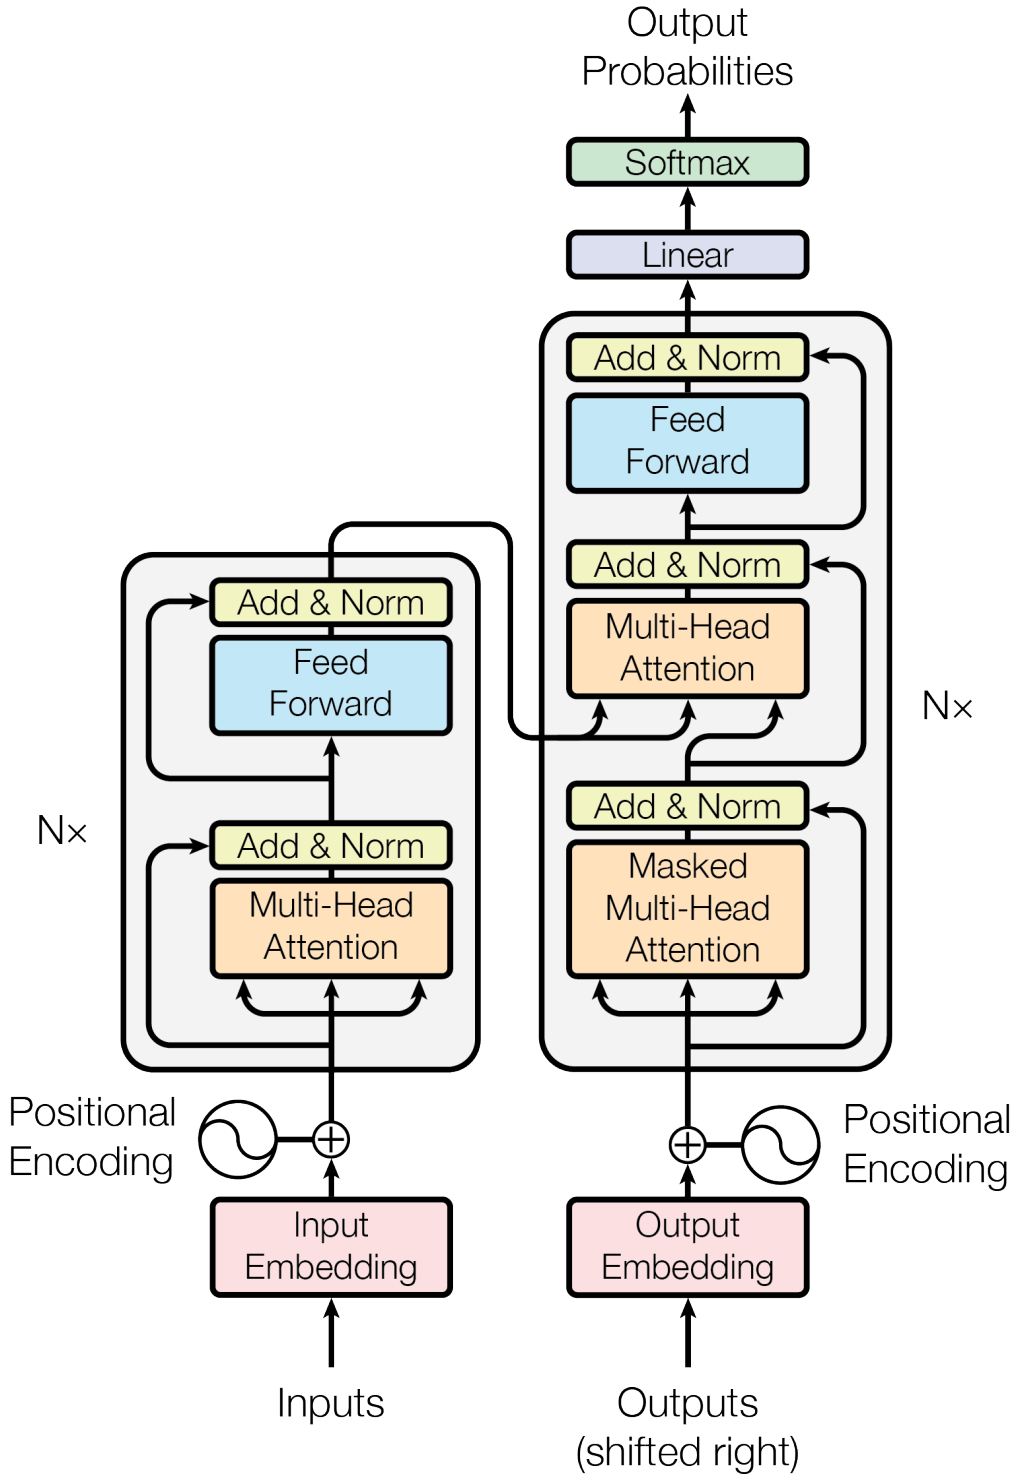
\includegraphics[width=0.5\textwidth]{Transformer model diagram}
\caption{Diagram depicting the architecture of the transformer model from \citet{AttentionIsAllYouNeed}.}
\end{figure}
\subsection{Problems solved by transformers}
The point of transformers was to overcome the problems faced by the previous state-of-the-art architectures while still including prominent aspects of the RNN and Convolutional Neural Network (CNN) models.

The RNN model has two notable weaknesses. First is its inability to learn long-term patterns, due to the exploding and vanishing gradient problems that occur during backpropagation.
Secondly, its recurrent connection is also a weakness. This is because it is not possible to compute the cell at time step $i$ until the cell at time step $i-1$ has been computed as information is propagated along a sequence.

In contrast, one of the benefits of CNNs is that they can be computed concurrently. However, unlike RNNs, they are unable to learn even short-term patterns. The size of the patterns they can learn is limited by their architecture.

Transformers attempt to feature the best of both techniques.
Transformers can model dependencies over the whole range of the input sequence as easily they can model neighboring sequences. And there are no recurrent connections, allowing efficient computation using parallelization. This is facilitated through the use of the self-attention mechanism.\cite{TransformersScratchPeterbloem}


\subsection{Self-attention Mechanism}
A self-attention mechanism is a sequence to sequence operation. This means that the input is a sequence of vectors $x_{1},x_{2},\ldots, x_{t}$, and the output is also a sequence of vectors $y_{1},y_{2},\ldots, y_{t}$.
These vectors all have dimension $k$.

To get the output vector $y_{i}$, the operation takes a weighted average over all input vectors.
$$
y_{i}=\sum_{j}w_{ij}x_{j}
$$
Here, $j$ indexes over the whole sequence, and the sum of all the weights in the sequence is one.
The weight $w_{ij}$ is derived from a function over $x_{i}$ and $x_{j}$.
This could, for example, be the dot product:
$$
w'_{ij}=x_{i}^Tx_{j}
$$
where $x_{i}$ is the input vector at the same position as the current output vector $y_{i}$.
The next output vector has a completely different series of dot products, and therefore a different weighted sum.

As the dot product can result in values between negative and positive infinity, the softmax activation function is used to map values to the interval $[0,1]$, and to ensure that they sum to $1$ over the entire sequence:
$$
w_{ij}=\frac{e^{w'_{ij}}}{\sum_{j}e^{w'_{ij}}}
$$
For maximum efficiency, computations are vectorized as much as possible. The resulting calculations become:
\begin{gather}
W'=X^TX\\
W=\text{softmax}(W')\\
Y^T=WX^T
\end{gather}\cite{TransformersScratchPeterbloem}


\subsection{How transformers work}
Transformers, as mentioned, primarily use self-attention. This forms the basis of the architecture.

There are several different variations of the transformer architecture, and the following is just one such variant.

First, the transformer block applies self-attention. Then it does layer normalization, after which it applies a feed forward network. The feed forward network here is a single MLP applied independently to each vector. And lastly, another layer normalization is applied.

The network may become permutation invariant, meaning the output will not change despite reordering. In the context of natural language processing, the ordering of the words in the input sentence would not matter. This can be detrimental to the training process, as it means the model is not learning the dependencies between words---positions matter. If every word in this paper were ordered alphabetically, it would not make much sense.

To solve this, one can use positional embeddings or positional encodings.

With positional embedding, the position of the word in the sentence is embedded. For this to work during training, sequences of every length would need to be seen, otherwise, the relevant positional embeddings do not get trained.

Positional encodings work in a similar fashion, except the positional vectors are not learned.
Instead, a function is chosen $f:\mathbb{N}\rightarrow\mathbb{R}^k$ that maps the positions to real-valued vectors. The network is left to figure out how to interpret these.\cite{TransformersScratchPeterbloem}
\subsection{Training}\label{sec:training}
In order to train the models, we used Deepnote\cite{deepnote} to achieve similar hardware performance on the training of all the models used for this project. 
The training was done using individual Python notebooks contained in a project on Deepnote, in order to allow easy collaboration between the authors.

The data used are open source and was collected on Kaggle\cite{kaggle}. It was provided by individual contributors for free use.
The data came from arbitrary cities of the world. 
It should be noted that we cannot verify the legitimacy of the data, the main objective was simply to gather datasets that were representative and meaningfully large to train the models on. 
The training of each model used arbitrary settings for the batch sizes, hyperparameters, learning rates and dropout rates. Similarly, no optimization algorithms were implemented in order to identify the optimal settings. 

Once the models have been trained, they are serialized using the Python \texttt{pickle} module.
This module converts the data and the Python objects into a byte stream which is stored in a file.
The process of serializing Python objects is known as pickling. 
This allows us to export the trained models from Deepnote, the first component in our pipeline, and onto the server used in the web application, the second component in our pipeline, as previously shown in figure \ref{fig:architecture diagram}.\cite{pickle_documentation}
\subsection{Web application}
Once the models have been trained, 

\section{Experiments \& Analysis}\label{sec:ExpRes}
\label{sec:ExpRes}

\begin{table}[]
\begin{tabular}{|l|r|r|r|r|}
\hline
\multicolumn{1}{|c|}{Models} & \multicolumn{1}{c|}{Austin} & \multicolumn{1}{c|}{Bangladesh} & \multicolumn{1}{c|}{Delhi} & \multicolumn{1}{c|}{Szeged} \\ \hline
GRU                          &                             &                                 & 0.0038                     &                             \\ \hline
LSTM                         &                             &                                 & 0.0038                     &                             \\ \hline
MLP                          & 5.2465                      & 0.7421                          & 1.6709                     & 1.31                        \\ \hline
RNN                          &                             &                                 & 0.0594                     &                             \\ \hline
Transformer                  &                             &                                 &                            &                             \\ \hline
\end{tabular}
\end{table}

\section{Conclusion}

%\section*{Acknowledgment}

\bibliographystyle{IEEEtranN}
\bibliography{bib/bib}

\appendix
%\input{appendix/...}

\end{document}